\documentclass{article}
\usepackage{graphicx} % Required for inserting images
\usepackage{caption}
\usepackage{subcaption}

\title{ASN2}
\author{William Grimmer, Jack Formato, Victoria Shelton}
\date{October 2024}

\begin{document}

\maketitle

\section{Design}
For our design we chose to do a layered architecture with a three tiered architecture model. It will have the GUI as the top layer, the application as the middle layer and the database as the bottom layer. We chose this as it works well with JavaScript and although MVC is commonly used we felt as if it would be easier to learn and understand layered architecture.

\subsection{Language}
For our language we will use JavaScript as we understand it is one of the premier languages for web applications and has tons of frameworks and libraries that support it such as Node and React. In addition Victoria has also worked with the language before which will help significantly with the learning curve.

\subsection{Frameworks/Libraries}
For our Frameworks and Libraries we will almost certainly use Node.js and React.js. Node.js is what allows for server side JavaScript hosting and will be necessary in order to create a web application. React.js helps to build user interfaces and the front end for web applications and will be very useful. For our testing framework we will be using Jest which is the newest and most common testing framework for JavaScript.

\subsection{Database}

For our Database we will use MySQL. We chose a SQL database over a noSQL version as Will and Jack are familiar with SQL from taking DBMS with Dr. Rocha. For that same reason we will use MySQL as our choice of SQL database as once again we are familiar with it.

\begin{figure}[h]
\centering
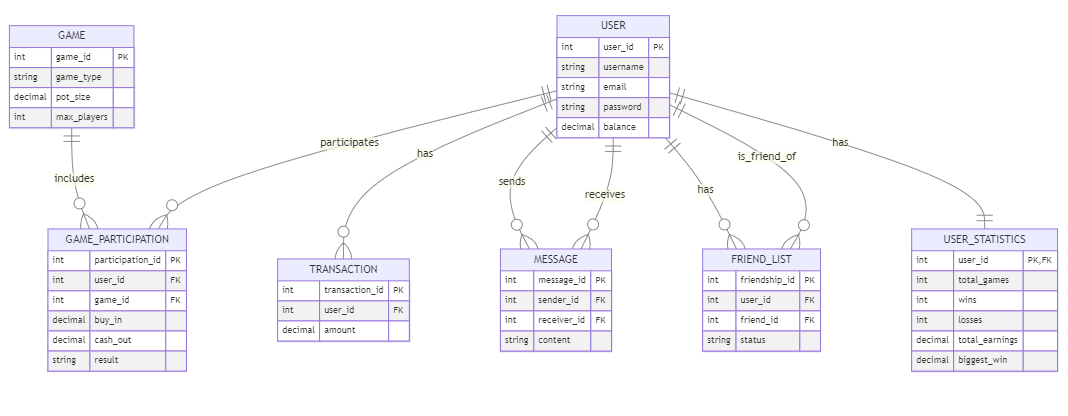
\includegraphics[width=\linewidth]{ERD.png}
\caption{\label{fig:erd}The Entity Relations Diagram for SQL.}
\end{figure}

\newpage
\subsection{coding standards}
For our coding standards we will follow Agile development and work iteratively in coding sprints. The goal is to prioritize working code and not commit anything that covers less than 70\% of test cases. Additionally we will use CamelCase as a naming convention to ensure consistency throughout the code. 


\section{UML}
Figure \ref{fig:uml} is our UML Diagram. This illustrates the class relationships in our project. Users will have Messages and UserStats. We have an Admin class which will extend. Admins, unlike normal Users, will be able to change a User's password. The Game Class has a Host, Players and a Deck. A Player will have a user, in order to add balance and update stats. A deck will be composed of Cards which are dependent on the deck and only exists with it. Players will have a hand, which consists of cards. A game will also have bots. Just like Players, Bots have a hand. These relationships should allow the program to run smoothly and efficiently.

\begin{figure}[h]
\centering
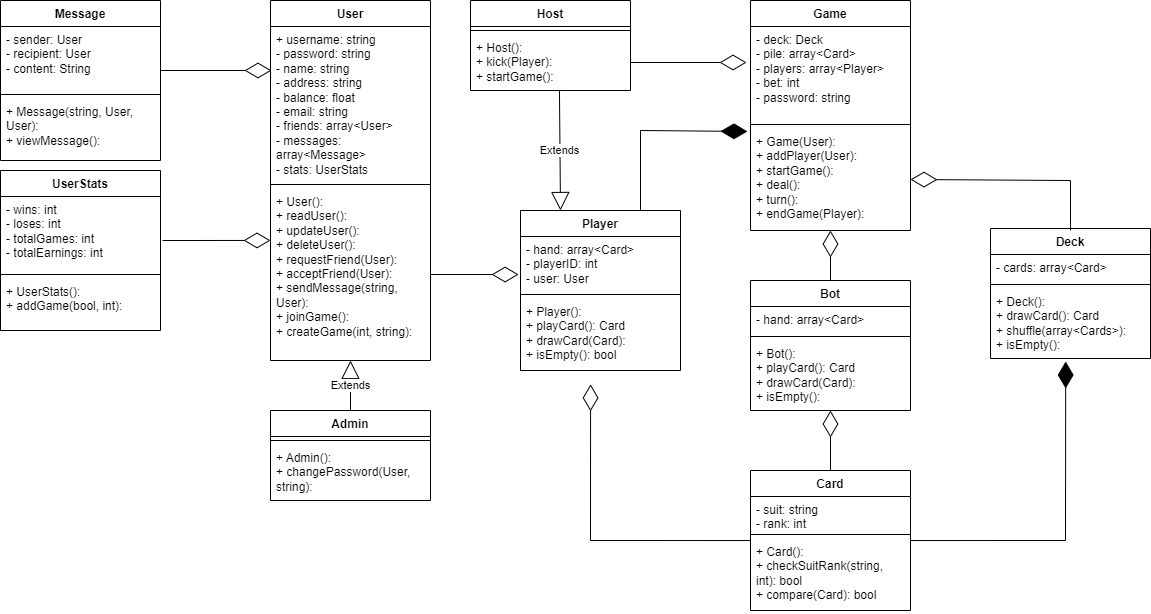
\includegraphics[width=\linewidth]{Crazy8sUML.png}
\caption{\label{fig:uml}High-level OOA UML Class Diagram}
\end{figure}

\section{Website UI Mockup}
\begin{figure}[h]
\centering
\begin{subfigure}{0.5\textwidth}
  \centering
  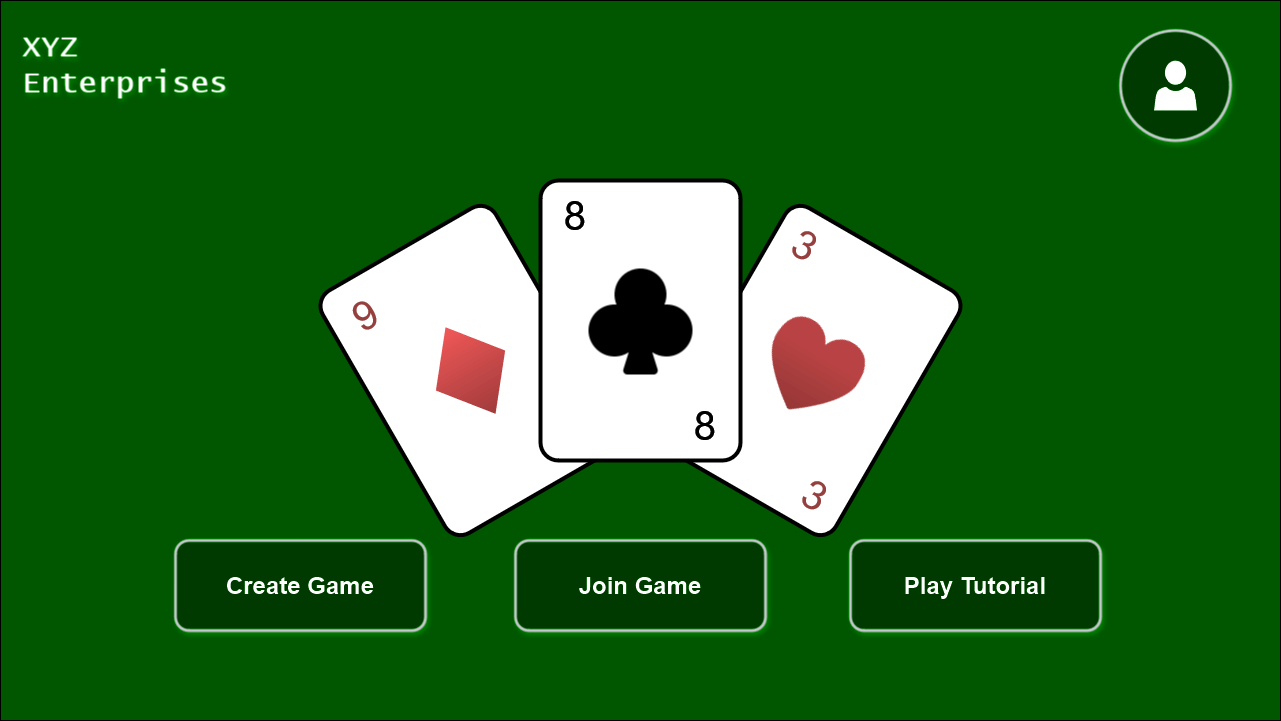
\includegraphics[width=.99\linewidth]{Menu.png}
  \caption{\label{fig:menu}The main menu.}
\end{subfigure}%
\begin{subfigure}{0.5\textwidth}
  \centering
  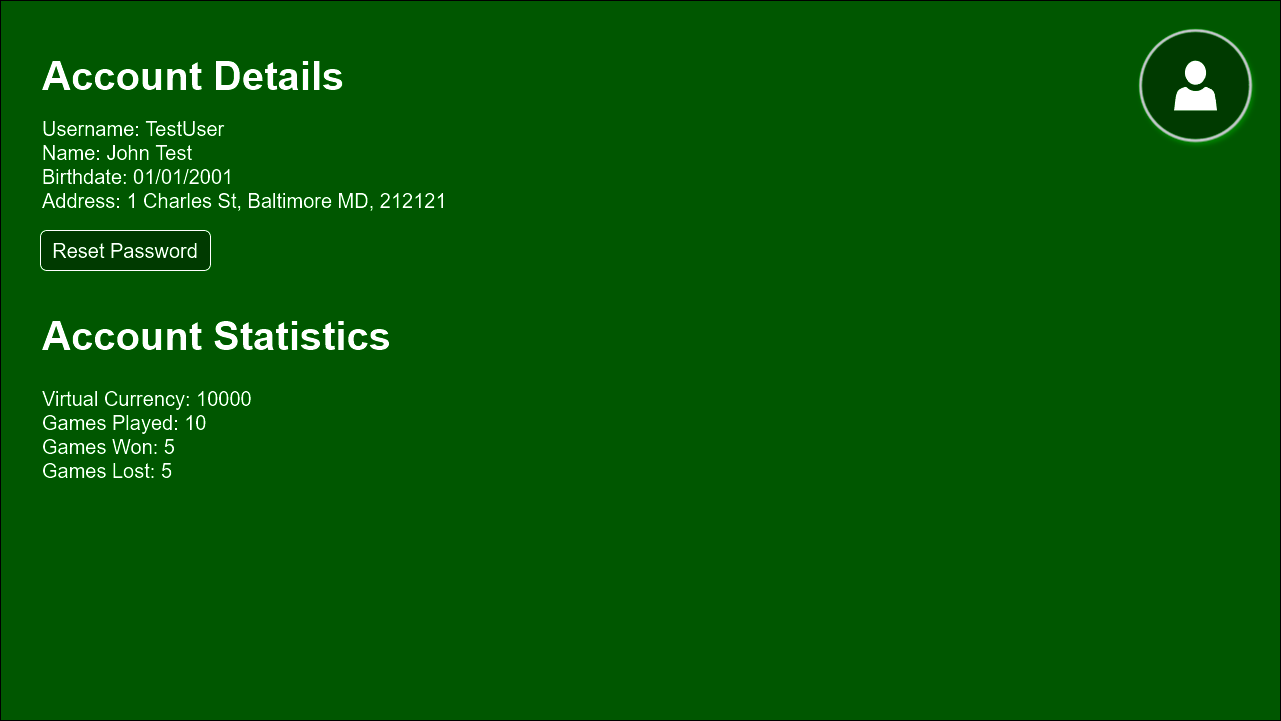
\includegraphics[width=.99\linewidth]{Account.png}
  \caption{\label{fig:account}The account menu.}
\end{subfigure}
\begin{subfigure}{0.5\textwidth}
  \centering
  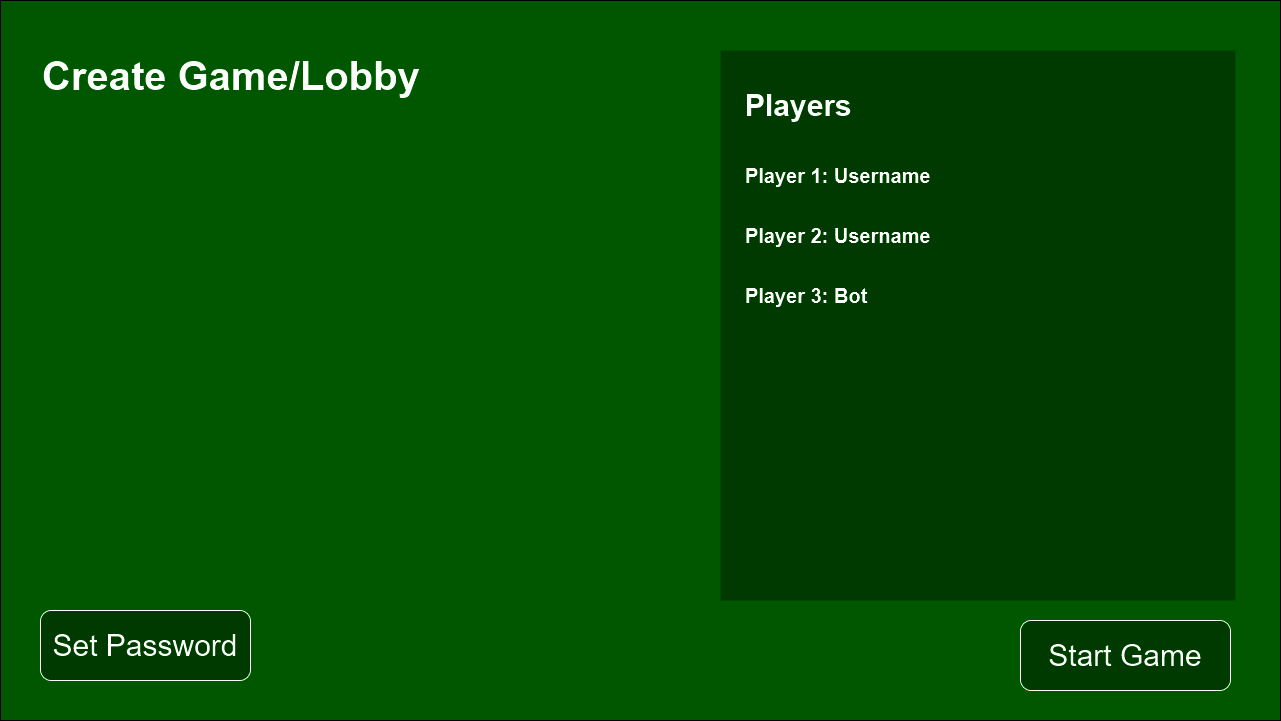
\includegraphics[width=.99\linewidth]{Create.png}
  \caption{\label{fig:create}The create game menu.}
\end{subfigure}%
\begin{subfigure}{0.5\textwidth}
  \centering
  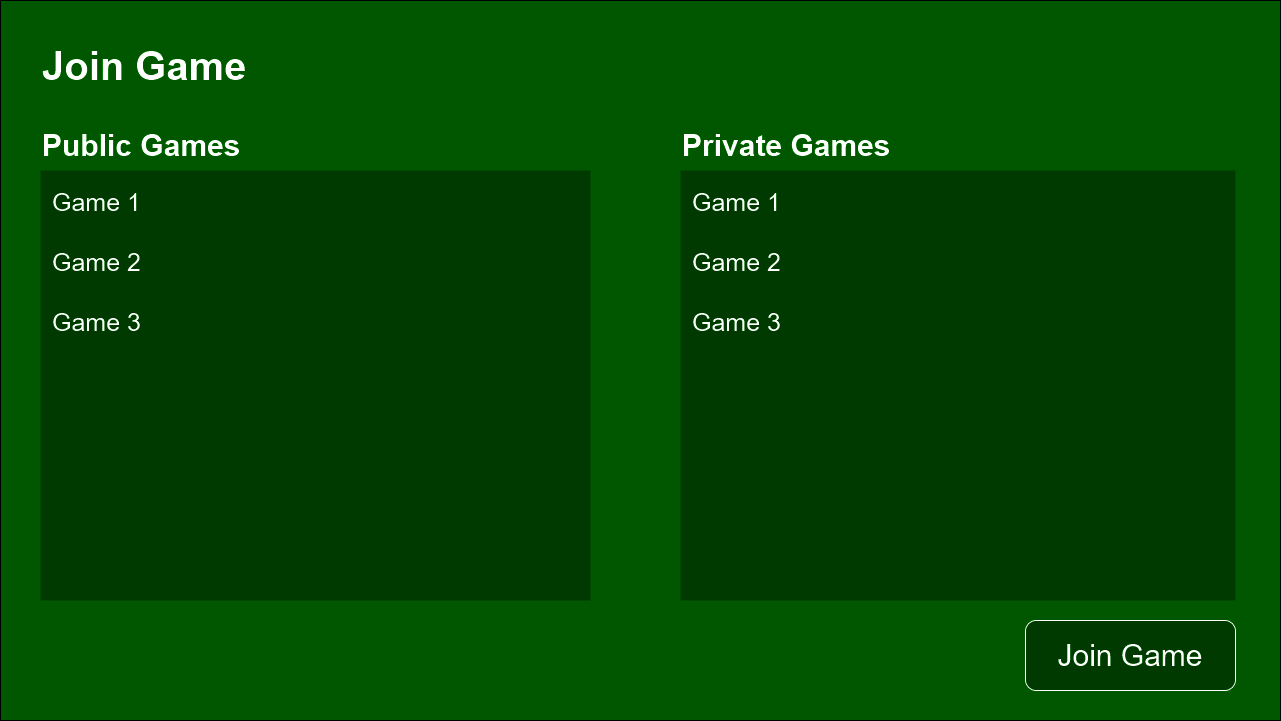
\includegraphics[width=.99\linewidth]{Join.png}
  \caption{\label{fig:join}The join game menu.}
\end{subfigure}
\begin{subfigure}{0.5\textwidth}
  \centering
  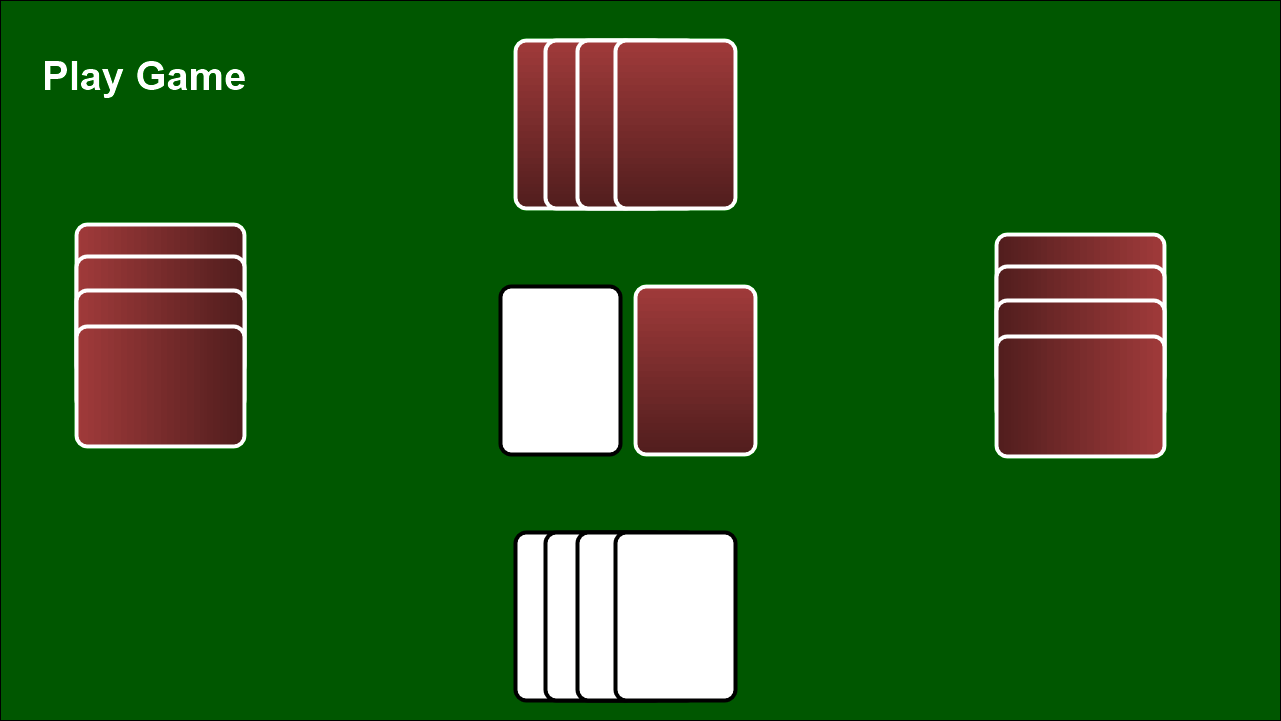
\includegraphics[width=.99\linewidth]{Game.png}
  \caption{\label{fig:game}The game menu.}
\end{subfigure}%
\begin{subfigure}{0.5\textwidth}
  \centering
  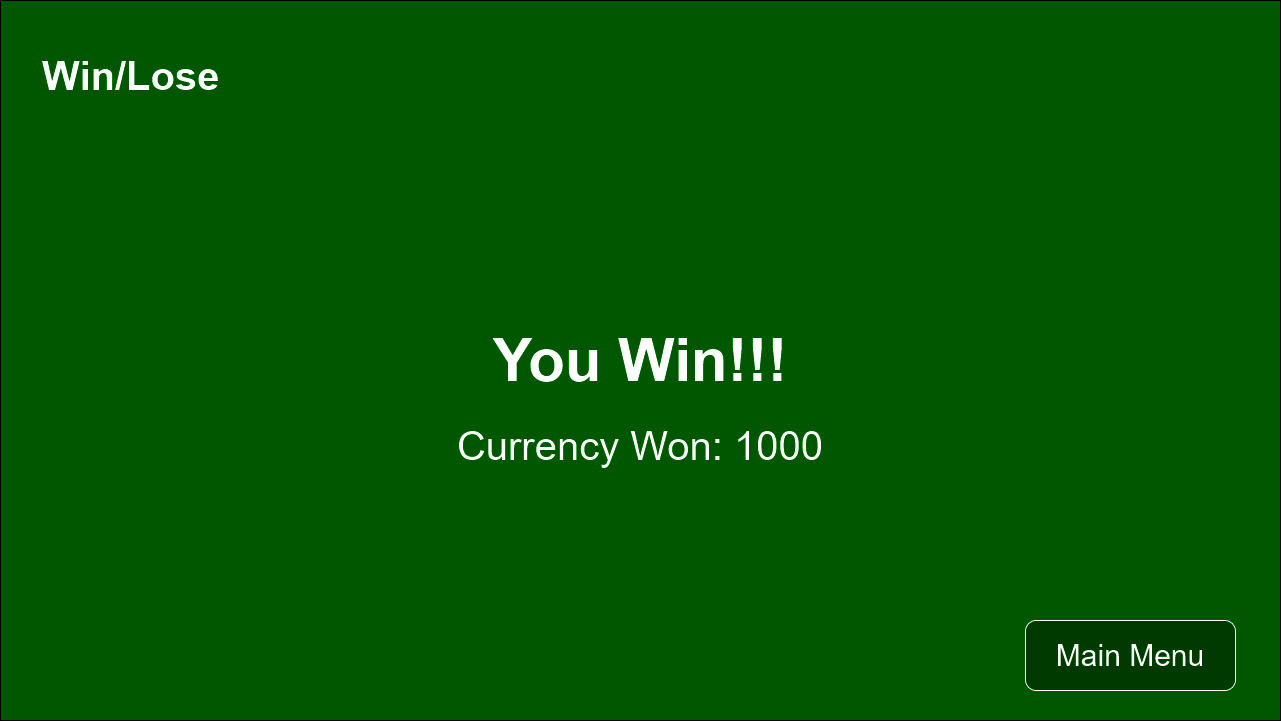
\includegraphics[width=.99\linewidth]{End.png}
  \caption{\label{fig:end}The end screen.}
\end{subfigure}
\end{figure}

The UI for the website should be simple and intuitive. For the main page (see Figure \ref{fig:menu}), the user has four options: create a game, join a game, play the tutorial, or check their account. The account menu page (see Figure \ref{fig:account}) allows users to check their account information and update their password. The create game page in Figure \ref{fig:create} allows users to host a game, set a password, manage players, etc. Players can also join games through the join game page in Figure \ref{fig:join}. When players are in a game, they see the screen in Figure \ref{fig:game}. Lastly, when a game ends, players will see the end screen in Figure \ref{fig:end}, which shows a message based on whether they win or lose and allows them to return to the main screen.

\end{document}
